%%%%%%%%%%%%%%%%%%%%%%%%%%%%%%%%%%%%%%%%%%%%%%%%%%%%%%%%%%%%%%%%%%%%%%%%%%%%%%%%
% Author : Evgenii Shiliaev, Tomas Polasek (template)
% Description : Seventh exercise in the Introduction to Game Development course.
%   It deals with the creation of a Game Design Document, presenting a short 
%   pitch for a potential game project.
%%%%%%%%%%%%%%%%%%%%%%%%%%%%%%%%%%%%%%%%%%%%%%%%%%%%%%%%%%%%%%%%%%%%%%%%%%%%%%%%

\documentclass[a4paper,10pt,english]{article}

\usepackage[left=2.50cm,right=2.50cm,top=1.50cm,bottom=2.50cm]{geometry}
\usepackage[utf8]{inputenc}

% Hyper-Text References
\usepackage{hyperref}
\hypersetup{colorlinks=true, urlcolor=blue}

% Drawing Images and Graphs
\usepackage{tikz}
\usepackage{pgfplots}

% Page Utilities
\usepackage{graphicx}

% Image Sub-Captions
\usepackage{subcaption}

% The whole document not to be indented
\setlength\parindent{0pt}

% Some muted warnings
% chktex-file 18
% chktex-file 24
% chktex-file 44

% Quotes fixing
\usepackage[english]{babel}
\usepackage[autostyle, english = american]{csquotes}
\MakeOuterQuote{"}

\newcommand{\ph}[1]{\textit{[#1]}}

\title{%
Game Pitch Document%
}
\author{%
Evgenii Shiliaev (xshili00)%
}
\date{}

\begin{document}

\maketitle
\thispagestyle{empty}

{%
	\large

	\begin{itemize}

		\item[] \textbf{Title:} \ph{Madness League}

		\item[] \textbf{Genre:} \ph{Action Racing game}

		\item[] \textbf{Style:} \ph{3D Realistic Art Style}

		\item[] \textbf{Platform:} \ph{PC, Xbox One/Series consoles, PlayStation 4/5 consoles}

		\item[] \textbf{Market:} \ph{Arcade-racing games audience / 13--40 years}

		\item[] \textbf{Elevator Pitch:} \ph{Multiplayer action arcade-racing game with power-ups and game-changing mutators}

	\end{itemize}

}

\subsection*{Introduction}
Madness League is a multiplayer action arcade racing game with a vehicle and environment destruction system.
During the race, players (up to 16) can collect power-ups and choose game-changing mutators by completing in-race challenges.

\subsection*{Background}
The main inspiration of core gameplay is the arcade machine in the mall of Kirov city, Russia.
Unfortunately, it is not possible anymore to find out its name, and the game hasn't a PC port.
It was about crazy off-road monster truck racing with \emph{Moorhuhn Kart}-like power-ups on nature tracks with immense sea-level changes.
The mutators were inspired by \emph{Move Or Die} game.
They significantly change game rules, controls, and even the core game mechanics.
The vehicle and environment destruction system was inspired by \emph{Flatout 2} because destruction is fun, especially with good physics.

\subsection*{Setting}
In 2025, the most popular QroakToker\footnote{\textbf{QroakTok} is the one and only social network, the meta social media.} started the "Disabled Airbag" show about insane racing tournaments for people who have nothing to lose.
Participants can be insolvent businessmen or crazy destitute people who are greedy for any opportunity to earn money. They get in the derby cars or monster trucks to meet themselves in savage races.
If they survive the qualifying, they will have a chance to change their lives in the true madness.

\subsection*{Genre}
\emph{Madness League} is an action game.
The player can damage opponents' vehicles by rushing into them at high speed or by using power-ups and tools during the route.
The game is arcade. It isn't about realism but fun, chaos, and fun chaos.
As more mutators are in the game, the more difficult it is to reach the finish but more fun.
The game is not about the story but pure gameplay.
And finally, \emph{Madness League} is a racing.
No matter what just push the pedal to the metal and be first.

\subsection*{Features}
The main feature of the game is the mutators (Table~\ref{tab:mutators}).
Unlike the power-ups, they modify the whole game session by changing the rules.
Many mutators and their combinations will make the game fun and hugely replayable.
The other significant feature is the AI of the enemies because they should be "clever" enough to challenge the players.
It is not acceptable to let computer opponents use dirty tricks, which are in other racing games.
The racing tracks' verticality will make them extremely dangerous and literally breathtaking.
The combination of these three main features makes the game unique among other already existing games on chosen platforms.
The target audience is grown-up \emph{Mario Kart} and \emph{Crash Team Racing} fans, \emph{Flatout 2} fans, and other casual players, especially on PC because there isn't any similar game to \emph{Madness League}.

\begin{figure}[h]

	\centering

	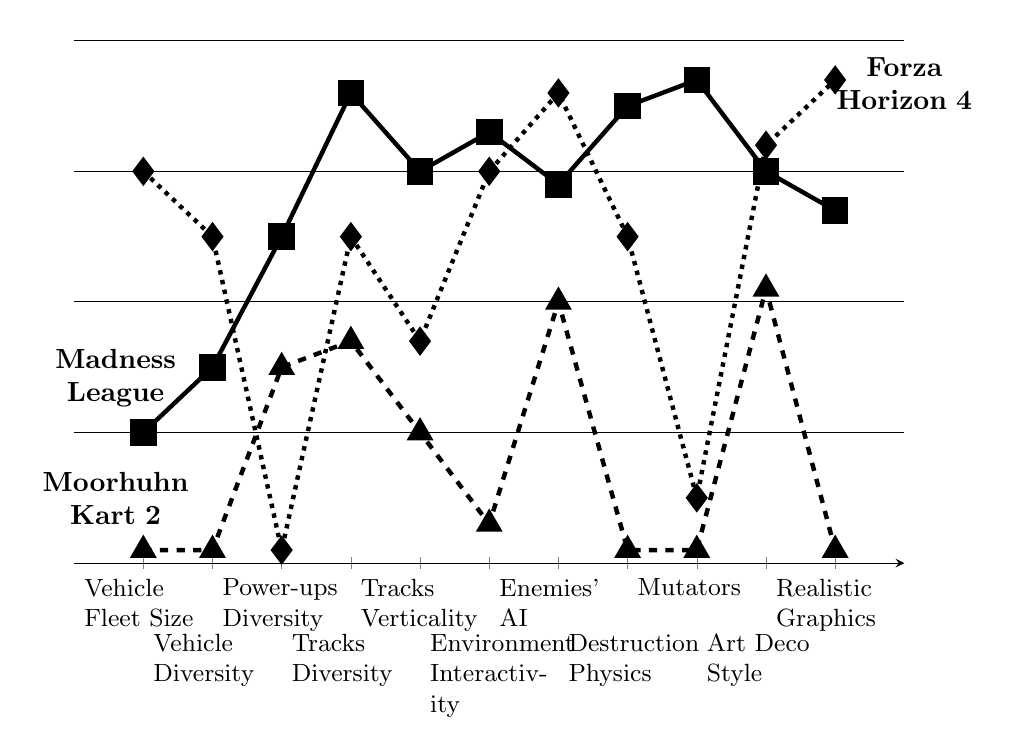
\begin{tikzpicture}[remember picture]%
		\begin{axis}[
				domain=0:1,
				clip=false,
				ymin=0, xmin=0, ymax=4.1, xmax=12,
				xtick={1,2,...,11},
				yticklabels={},
				xticklabels={Vehicle Fleet Size, Vehicle Diversity, Power-ups Diversity, Tracks Diversity, Tracks Verticality, Environment Interactivity, Enemies' AI, Destruction Physics, Mutators, Art Deco Style, Realistic Graphics},
				xticklabel style={yshift={-mod(\ticknum, 2) * 2em}, text width=1.5cm, font=\small},
				y tick style={draw=none},
				x axis line style={|-|},
				y axis line style={draw=none},
				axis lines=middle,
				width=\linewidth,
				height=0.3\paperheight
			]
			\addplot [ultra thick, mark=square*, mark options={scale=2,solid}] coordinates {
					(1, 1.0)
					(2, 1.5)
					(3, 2.5)
					(4, 3.6)
					(5, 3.0)
					(6, 3.3)
					(7, 2.9)
					(8, 3.5)
					(9, 3.7)
					(10, 3.0)
					(11, 2.7)
				} node[above, yshift=15pt, pos=0, yshift=-10pt, xshift=-10pt, text width=2cm, align=center] {\textbf{Madness League}};

			\addplot [ultra thick, dashed, mark=triangle*, mark options={scale=2,solid}] coordinates {
					(1, 0.1)
					(2, 0.1)
					(3, 1.5)
					(4, 1.7)
					(5, 1.0)
					(6, 0.3)
					(7, 2.0)
					(8, 0.1)
					(9, 0.1)
					(10, 2.1)
					(11, 0.1)
				} node[above, yshift=5pt, xshift=-10pt, pos=0, text width=2cm, align=center] {\textbf{Moorhuhn Kart 2}};

			\addplot [ultra thick, dotted, mark=diamond*, mark options={scale=2,solid}] coordinates {
					(1, 3.0)
					(2, 2.5)
					(3, 0.1)
					(4, 2.5)
					(5, 1.7)
					(6, 3.0)
					(7, 3.6)
					(8, 2.5)
					(9, 0.5)
					(10, 3.2)
					(11, 3.7)
				} node[above, yshift=-15pt, xshift=25pt, pos=1, text width=2cm, align=center] {\textbf{Forza Horizon 4}};

			\draw [] (axis cs:{0,1}) -- (axis cs:{12,1});
			\draw [] (axis cs:{0,2}) -- (axis cs:{12,2});
			\draw [] (axis cs:{0,3}) -- (axis cs:{12,3});
			\draw [] (axis cs:{0,4}) -- (axis cs:{12,4});
		\end{axis}
	\end{tikzpicture}

	\caption{Value graph for \emph{Madness League}, \emph{Moorhuhn Kart 2}, and \emph{Forza Horizon 4}.}
	\label{Fig:ValueGraph}

\end{figure}

\begin{table}[h]
	\centering
	\begin{tabular}{
			p{\dimexpr.32\linewidth-2\tabcolsep-1.3333\arrayrulewidth}
			p{\dimexpr.68\linewidth-2\tabcolsep-1.3333\arrayrulewidth}}
		\textbf{Name}          & \textbf{Description}                   \\ \hline
		From Zero to Hero      & The last player becomes the first.
		The rest of the players disappear from the leaderboard.
		They must update their position by touching the first player.   \\ \hline
		Death Zone             & A moving zone appears.
		All players must be in there, otherwise, they will take damage.
		There is an option when the center of the area is a player.     \\ \hline
		Back to Roots          & The finish point is now behind.
		Players must reroute in the opposite direction.                 \\ \hline
		Learn to Drive. Again. & Players can go forward only backwards.
		Difficult one.                                                  \\ \hline
	\end{tabular}
	\caption{Some mutators examples}
	\label{tab:mutators}
\end{table}

\subsection*{Platform}
The game will release on PC, 8th and 9th generation consoles of Microsoft and Sony.
\emph{Madness League} can be ported to Nintendo consoles later to take away some Mario Kart fans from Nintendo.

\end{document}
